\documentclass[12pt]{report}
\usepackage{flushend}
\usepackage{graphicx}
\usepackage[noadjust]{cite}
\usepackage[toc,acronym,description,sort=def]{glossaries}
\usepackage{sectsty}
\usepackage{setspace}
\usepackage{enumerate}
\usepackage{IEEEtrantools}
\usepackage{paralist}
\usepackage{chngcntr}
\usepackage{ftnxtra}
\usepackage{amsmath}
\usepackage{algorithm}
\usepackage{url}
\usepackage{array}
\usepackage{listings}
\usepackage[noend]{algpseudocode}
\counterwithout{footnote}{chapter}
\algnewcommand{\LeftComment}[1]{\Statex \(\triangleright\) #1}
\renewcommand{\bibname}{References}
\renewcommand{\algorithmicrequire}{\textbf{Input:}}
\renewcommand{\algorithmicensure}{\textbf{Output:}}
\chapterfont{\centering}
\pagestyle{headings}
\onehalfspacing

%************Glossary*************%

\makeglossaries

\newglossaryentry{dna}
{
    name=DNA,
    description={Deoxyribo Nucleic Acid, a molecule that codes genetic instructions in living organisms. It is a \emph{string} of 4 `nucleotides' - Nitrogen containing bases: Cytosine (C), Guanine (G), Adenine (A), and Thymine (T)}
}

 
%********End of Glossary**********%

\begin{document}

\begin{titlepage}
\begin{center}
\vspace{1cm}
\huge
\textbf{Extending eXpOS to Multi-core Environment}\\

\normalsize
\textbf{CS4090 Project Final Report}\\
\vspace{1cm}
\emph{Submitted by}\\        
\vspace{0.5cm}
\begin{tabular}{ccc}
\textbf{Arun Joseph}&& \textbf{B150102CS}\\
\end{tabular}\\
\vspace{0.8cm}
\textbf{Under the Guidance of\\Dr. K. Muralikrishnan}\\
\vspace{0.8cm}
\begin{center}
 
\includegraphics[width=0.2\textwidth]{nitc-logo.png}
\end{center}
\vspace{0.8cm}
\textbf{Department of Computer Science and Engineering}\\
\textbf{National Institute of Technology Calicut}\\
\textbf{Calicut, Kerala, India - 673 601}\\
\vspace{0.8cm}
\textbf{April 26, 2019}
\end{center}
\end{titlepage}
\pagenumbering{roman}
\begin{spacing}{1.01}
{
\thispagestyle{empty}

\fontsize{14}{14}\selectfont
\centering{\MakeUppercase{\textbf{National Institute of Technology Calicut, Kerala, India - 673 601}}} \\
\vspace*{0.5cm}
\fontsize{12}{12}\selectfont
\centering{\MakeUppercase{\textbf{DEPARTMENT OF COMPUTER SCIENCE AND ENGINEERING}}} \\
\begin{figure}[ht]
{\centering {
\includegraphics[width=0.2\textwidth]{nitc-logo.png}}\par}
\end{figure}
2019\\
\vspace{0.5cm}
\fontsize{14}{14}\selectfont
\textbf{\centering{CERTIFICATE}}\\
\vspace{0.25cm}
\fontsize{12}{12}\selectfont
\onehalfspacing{\textit{Certified that this is a bonafide record of the project work titled}}\\
\vspace*{0.25cm}
\textbf{\MakeUppercase{Extending eXpOS to Multi-core Environment}}\\
\vspace*{0.25cm}
\onehalfspacing{\centering{\textit{done by}}}\\
\vspace*{0.25cm}
\begin{tabular}{ccc}
\textbf{Arun Joseph}\\
\end{tabular}\\
\vspace*{0.25cm}
\onehalfspacing{ \textit{\centering{of eighth semester B. Tech in partial fulfillment of the requirements for the award of the degree of Bachelor of Technology in Computer Science and Engineering of the National Institute of Technology Calicut}}}\\
\vspace*{2cm}
\noindent{
\begin{tabular}{p{4.5cm}cp{4.5cm}}
\textbf{Project Guide}  & \hfill \textbf{Head of Department} \\
Dr. K. Muralikrishnan & \hspace{5cm} Dr. Saleena N\\
Associate Professor & \hspace{5cm} Associate Professor\\
 & & \\
 & & \\
  & & \\

\end{tabular}
}
}
\chapter*{DECLARATION}
I hereby declare that the project titled, \textbf{Extending eXpOS to Multi-core Environment}, is my own work and that, to the best of my knowledge and belief, it contains no material previously published or written by another person nor material which has been accepted for the award of any other degree or diploma of the university or any other institute of higher learning, except where due acknowledgement and reference has been made in the text.\\

\vspace{2cm}
\noindent{
\begin{tabular}{p{8cm}p{6cm}}
Place : & Signature : \\
Date : & Name : \\
 & Reg. No. : 
\end{tabular}
}
\newpage 

\begin{abstract}
Project eXpOS (eXperimental Operating System) is an on-line educational platform which helps undergraduate students to learn the working of an operating system. It is an instructional tool for students to learn and implement OS data structures and functionalities in a few months. This project aims at extending eXpOS to a dual-core environment.
\end{abstract}

\chapter*{\rm \large \bf ACKNOWLEDGEMENT}
\paragraph{}
I would like to express my deepest appreciation to all those who helped and supported me in completing this project. I am highly indebted to my project guide, Dr. K. Muralikrishnan, for his constant guidance and supervision in guiding me through this project.

\paragraph{}
I would like to express my gratitude towards Dr. Saleena N, Head of Department of Computer Science and Engineering, and Dr. Lijiya A, Project Coordinator, for providing me this platform. I would like to thank the eXpOS team for their past contributions in the earlier versions of this project.

\paragraph{}
I would also like to thank Rohith Vishnumolakala for helping out in the initial stages of this project. Lastly, I would like to thank my juniors in OS Laboratory for identifying and reporting issues in the previous version of this project.
\vspace{4.0mm}

\tableofcontents
\addtocontents{toc}{\vskip-30pt}
\end{spacing}

\listoffigures
\listoftables
\vspace{-2 em}
\printglossary[nonumberlist]

\chapter{Introduction}
\pagenumbering{arabic}
Project eXpOS~\cite{expos} is an educational platform for learning and developing a simple operating system on the XSM (eXperimental String Machine) Simulator. Earlier XOS~\cite{xos} (previous version of eXpOS) was used, which was replaced with the current updated version.

\paragraph{}
eXpOS has features like multi-programming, process management, disk management, demand paging, synchronization and multi-user capabilities. The basic machine model consists of memory, disk and CPU. There are two privilege levels of execution, namely user mode (unprivileged) and kernel mode (privileged). The virtual address space of a process is divided into library, heap, code and stack. The Operating System consists of 15 interrupts, 26 system call routines, 8 modules, handlers for hardware interrupts like timer, disk and console, and exception handling. It also contains OS data structures like Process Table, Page Table, Open File Table, etc.

\paragraph{}
The eXpFS (eXperimental File System) provides a file abstraction for the programmer. It consists of three types of files - the root, data files and executable files. The ABI (Application Binary Interface) is the interface between a user program and the kernel. The support tools for eXpOS includes XFS Interface, ExpL (Experimental Language) compiler,  SPL (System Programmer's Language) compiler and XSM debugger.


\section{Literature Survey}
There are several Operating Systems developed for educational purposes by different universities. Some of them are mentioned below.

\paragraph{}
The Xv6~\cite{ref-xv6} is a Unix-like teaching operating system developed for MIT's operating systems course. It is written in ANSI C and runs on multiprocessor x86 machine. It has multiprocessor support by handling concurrency with lock and threads, unlike special case solutions for uni-processors such as enabling/disabling interrupts.

\paragraph{}
XINU~\cite{ref-xinu} (Xinu Is Not Unix) is a student built operating system for understanding the inner workings of an OS developed at Purdue University. The course topics include memory management, scheduling, concurrent processing, device management, file systems, etc.

\paragraph{}
Nachos~\cite{ref-nachos} (Not Another Completely Heuristic Operating System) is an instructional teaching software developed by University of California, Berkeley. It consists of Machine, Threads and User Programs classes. The machine has registers, memory and CPU, and roughly approximates the MIPS architecture. The threads run in a virtual address space and has various states (ready, running, blocked, created) and methods (sleep, yield, fork). Nachos requires that code is in "Noff" format and a MIPS Simulator executes code for user program running on top of the Nachos Operating System.

\paragraph{}
Topsy~\cite{ref-topsy} (Teachable OPerating SYstem) is another small operating system desinged for teaching purposes at ETH Zurich. The system works on real x86 hardware.  

\paragraph{}
Other similar teaching operating systems include Minix~\cite{ref-minix}, GeekOS~\cite{ref-geekos}, TempOS~\cite{ref-tempos}, OS-161~\cite{ref-os161}, SimOS~\cite{ref-simos}, PintOS~\cite{ref-pintos}. The survey article~\cite{ref-survey1} reports that Nachos is the most popular among the systems discussed here. A recent survey~\cite{ref-survey2} indicates that the Xv6 system has gained popularity recently.


\section{Problem Definition}
The objective of the project are the following :-
\begin{itemize}
    \item Conduct a design review of the existing eXpOS architecture.
    \item To extend the existing XSM architecture to a dual core system with identical registers.
    \item Extend the eXpOS Operating System to run on the extended architecture utilizing the multi-processing facility.
    \item Design and implementation of support tools like compilers, assemblers, etc., for the extended machine architecture.
\end{itemize}

\chapter{Design}
This project focuses on improving the existing eXpOS system and adding multiprocessor support to the system. The first phase of the project reviewed the existing eXpOS system critically for design errors and proposing fixes to the design. Subsequently, enhancements the architecture and well as the OS to support multiprocessing is discussed.  

\section{Improvements to existing eXpOS Design}
A design review of the existing eXpOS architecture was done and the following modifications were introduced:
\begin{enumerate}
    \item 
    \textbf{Design error:} If the \emph{Fork} system call is called by a process which doesn't have heap pages, the heap pages will not be shared by the parent and the child as any subsequent page fault will allocate different pages for their heap and thus, violating the sharing semantics. 
    \newline
    \textbf{Fix:} The \emph{Fork} system call was modified to allocate heap pages (if not allocated before) for the parent and thus, child process will share the heap pages after forking. The Exception handler was modified to allocate both the heap pages when a page fault occurs due to heap, instead of one page.
    
    \item
    \textbf{Design error:} In the \emph{Fork} system call, the parent process first acquires a PCB entry by invoking the \emph{Get Pcb Entry} function in \emph{Process Manager}. It then calls \emph{Get Free Page} function in \emph{Memory Manager} to allocate 3 pages for Stack/User Area Pages for the child process. During the acquiring of the free pages, the parent process could go to WAIT\_MEM state (when free pages are not available), which may cause another process to acquire the same child process.
    \newline
    \textbf{Fix:} A new state called ALLOCATED was introduced and the child process is changed to ALLOCATED state after acquiring it.
    
    \item
    \textbf{Design error:} In the existing design of eXpOS, there was a possibility that a swapped out process will never be swapped in (a process is only swapped in when its state is READY) and resulting in only the idle process being scheduled.
    \newline
    \textbf{Fix:} A swapper daemon is introduced as a new process similar to the idle program, with PID=15, and the \emph{Pager Module} is called from the context of this process. This modification fixes the above problem, as there will always be two processes to perform the swap operation. To add fairness for the swapped out processes, if the TICK field of any swapped out process exceeds a threshold, that process is swapped in after swapping out another process in memory.
    
    \item
    \textbf{Design error:} During an exception, the machine didn't store the contents of EIP, EC, EPN and EMA registers and pushed the IP value on top of the user stack.
    \newline
    \textbf{Fix:} The exception handler hardware was corrected to perform the appropriate actions. The eXpOS roadmap and documentation were also updated for the same.

    \item Other modifications include:
    \begin{itemize}
        \item Corrections were done in the roadmap and documentation in accordance with the above changes in the eXpOS website.
        \item The user interface of the XFS-Interface was updated to the current eXpOS architecture.
        \item In XSM debugger, new commands like step n, list and watchpoints, and commands for displaying data structures were added, for easier debugging.
    \end{itemize}
\end{enumerate}

\section{NEXSM Architecture Specification}
NEXSM is an extension of the XSM architecture with a dual core feature. The machine has two identical cores with the same set of internal registers sharing a common memory. All registers in XSM are present in both the cores. Additionally, NEXSM cores contain an additional register called the \textbf{core flag}. A few additional privileged instructions provide primitives for synchronization between the two cores. One of the processors is called the \textbf{primary core} and the other called the \textbf{secondary core}. The machine can operate in two modes -- \textbf{active} mode and \textbf{reset} mode. In reset mode, the secondary is non-functional. The mode in which the machine operates can be controlled by the primary using a pair of special privileged instructions -- START and RESET.

\begin{figure}
    \centering
    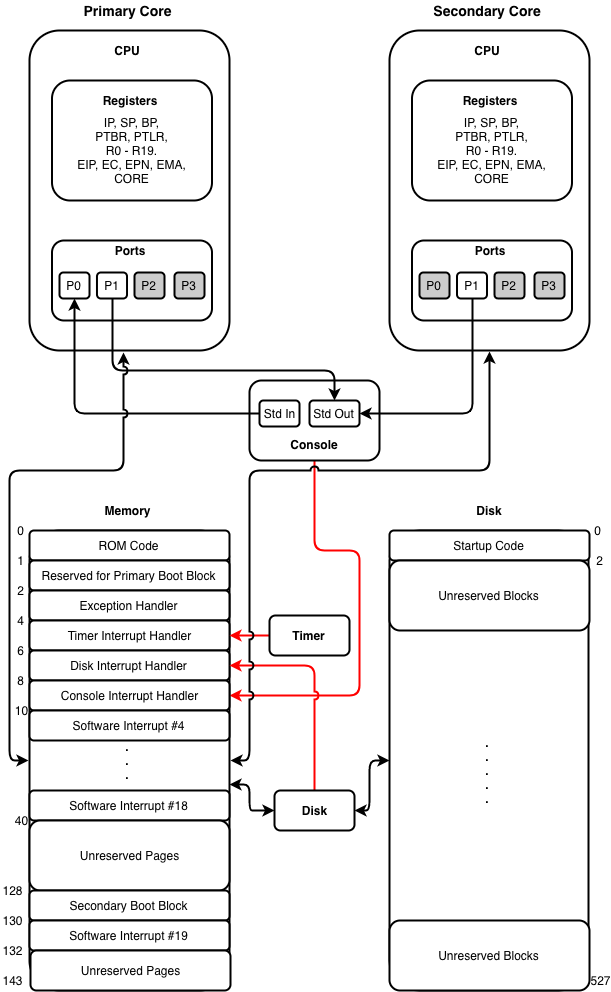
\includegraphics[scale=0.6]{nexsm_arch.png}
    \caption{NEXSM Architecture}
    \label{nexsm_arch}
\end{figure}

\subsection{Additional Registers}
The only additional register in NEXSM, that is not present in XSM, is the core flag (CORE). The core flag is a \textbf{read-only machine register}. The content of the core flag is set to 0 in the primary core and 1 in the secondary core. The core flag allows a program to test whether it is currently executing in the primary or the secondary.
\newline
\emph{Usage Example:} JZ CORE, [Address]

\subsection{Additional Privileged Mode Instructions}
\begin{itemize}
    \item{\textbf{Test and Set Lock}
    \newline \emph{Syntax:} TSL Rj, [loc]
    \newline \emph{Semantics:} The contents of the memory location (loc) is copied to register Rj. The value of [loc] is set to 1. This instruction is \textbf{atomic}. That is, when one of the cores is executing the TSL instruction, the memory bus is locked to avoid the other processor from simultaneously accessing [loc].}
    
    \item{\textbf{Dual-Core initialization}
    \newline \emph{Syntax:} START
    \newline \emph{Semantics:} If this instruction is executed by the primary while the machine is in reset mode, then secondary core starts parallel execution at the starting address of memory page 128 (physical address 65536). The START instruction is ignored if executed when the machine is in active mode.}
    
    \item{\textbf{Reset instruction}
    \newline \emph{Syntax:} RESET
    \newline \emph{Semantics:} The instruction, when executed in active mode sets the machine to reset mode.  The instruction is ignored if executed in active mode.}
\end{itemize}

\subsection{Disk Organization}
NEXSM has 16 additional blocks of disk space, with block numbers 512 to 527.

\subsection{Memory Organization}
NEXSM machine has 144 memory pages (as against 128 pages of XSM). The memory organization of pages 0 to 127 are exactly as in XSM. The organization of the remaining 16 pages are as follows:
\begin{itemize}
    \item Pages 128 and 129 are reserved for loading the bootstrap code for the secondary core.
    \item Pages 130 and 131 are reserved for an additional software interrupt INT 19.
    \item Pages 132 to 143 are available as free memory.
\end{itemize}

\subsection{Dual-Core Bootstrap}
\begin{enumerate}
    \item When powered on, the machine starts in reset mode. The primary core starts execution and the secondary core is non-functional. Here, the functioning is similar to XSM.
    \item When the machine is powered on, the primary executes a bootstrap code which loads the initialization code for the secondary core into memory page 128.
    \item The secondary core starts execution when the primary core executes a START instruction.
    \item Upon execution of the START instruction, the machine enters the active mode. The START instruction sets the IP value of the secondary core to physical address 65536 (page 128) and secondary core is powered on.
    \item When the machine is running in active mode, if a RESET instruction is executed by either the primary or the secondary, then the machine goes back to reset mode and the secondary stops execution.
\end{enumerate}

\subsection{Interrupts and Exceptions}
The way NEXSM machine enters privileged mode is similar to XSM, i.e., only when a software/hardware interrupt or exception occurs. The details are as follows:
\begin{enumerate}
    \item The disk and the terminal interrupts apply to the primary core only.
    \item Software interrupts, exceptions and timer interrupt applies to both the cores.
    \item NEXSM permits an additional software interrupt INT19.
\end{enumerate}


\section{eXpOS Design for NEXSM}
As NEXSM is only a dual-core extension XSM, the user interface of eXpOS undergoes no modifications. But the design of eXpOS changes when ported to the dual-core machine.

\subsection{Modifications to Application Interface}
The application interface of eXpOS undergoes minor modification when moving to NEXSM. The version of eXpOS running on NEXSM supports an additional software interrupt, INT 19. There are four system calls that gets mapped to INT 19 routine. Currently, these system calls are unused but could be used for testing future enhancements to the system. These are shown in Table~\ref{syscalls}.

\begin{table}[h!]
    \centering
    \begin{tabular}{|c|c|c|}
        \hline
        \textbf{System Call Name} & \textbf{Function Code} & \textbf{System Call Number} \\ [0.5ex]
        \hline
        Test4 & "Test4" & 100 \\
        \hline
        Test5 & "Test5" & 101 \\
        \hline
        Test6 & "Test6" & 102 \\
        \hline
        Test7 & "Test7" & 103 \\
        \hline
    \end{tabular}
    \caption{INT 19 System Call Interface}
    \label{syscalls}
\end{table}

\subsection{Disk Organization}
NEXSM disk has 16 additional disk blocks (block numbers 512 to 527). The Disk Organization of the new blocks is shown in Table~\ref{diskorg}.

\begin{table}[h!]
    \centering
    \begin{tabular}{|c|c|}
        \hline
        \textbf{Block Number} & \textbf{Contents} \\ [0.5ex]
        \hline
        512 - 513 & Secondary Bootstrap Code \\
        \hline
        514 - 515 & Interrupt 19 Routine \\
        \hline
        516 - 517 & Module 8: Access Control Module \\
        \hline
        518 - 519 & Module 9: TestA Module \\
        \hline
        520 - 521 & Module 10: TestB Module \\
        \hline
        522 - 523 & Module 11: TestC Module \\
        \hline
        524 - 527 & Unallocated \\
        \hline
    \end{tabular}
    \caption{Disk Organization}
    \label{diskorg}
\end{table}

\subsection{Memory Organization}
NEXSM has 16 additional pages of memory (pages 128 to 143). The Memory Organization is shown is Table~\ref{memorg}. The first four new pages are reserved by the machine. eXpOS reserves the next eight pages for storing OS code, while the remaining four pages are not used. Module 8 is called \textbf{Access Control Module} and contains code for synchronization between the two cores. Module 9, Module 10 and Module 11 are called TestA Module, TestB Module and TestC Module, respectively, and the present design doesn't use them.
The OS maintains an \textbf{Access Lock Table} to hold the access lock variables.

\begin{table}[h!]
    \centering
    \begin{tabular}{|c|c|c|}
        \hline
        \textbf{Block Number} & \textbf{Contents} & \textbf{Word Address} \\ [0.5ex]
        \hline
        57 & Access Lock Table & 29576 - 29583 \\
        \hline
        128 - 129 & Secondary Bootstrap Code & 65536 - 66559 \\
        \hline
        130 - 131 & Interrupt 19 Routine & 66560 - 67583 \\
        \hline
        132 - 133 & Module 8: Access Control Module & 67584 - 68607 \\
        \hline
        134 - 135 & Module 9: TestA Module & 68608 - 69631 \\
        \hline
        136 - 137 & Module 10: TestB Module & 69632 - 70655 \\
        \hline
        138 - 139 & Module 11: TestC Module & 70656 - 71679 \\
        \hline
        140 - 143 & Reserved for Future Use & 71680 - 73727 \\
        \hline
    \end{tabular}
    \caption{Memory Organization}
    \label{memorg}
\end{table}

\subsection{Design Policies}
\paragraph{}
The fundamental issue to be resolved while extending the OS to a dual-core machine is to ensure that concurrent updates of OS data structures from the two cores do not leave the OS in an inconsistent state. Here we impose a few simple to implement design level restrictions on the level of parallelism permitted so that a simple and comprehensible design is possible. The constraints imposed are the following:

\paragraph{}
\emph{\textbf{Policy 1:} Atomicity constraints:}
\begin{enumerate}
    \item A single process will never be scheduled simultaneously on both the cores. The scheduler will be designed to ensure this policy.
    \item Only one core will run scheduler code that involves updates to kernel data structures at a given time. This makes implementation of the first policy straight-forward.
    \item Only one core will be execute the critical section at a time. Upon entry into a system call the kernel checks whether the other core is running critical kernel code. If that is the case, then the kernel waits for the other core to finish the critical code before proceeding.
\end{enumerate}

\paragraph{}
\emph{\textbf{Policy 2:} Hold and Wait conditions:}
\newline
A process, after acquiring an access lock will quickly perform the required action and release the lock immediately, before being scheduled out. Moreover, a second access lock will be acquired only after releasing the first. These constraints ensure that there will be no hold and wait or circular wait for access locks.

\subsection{Access Lock Table}
An additional layer of access locking is required to ensure the atomicity constraint is satisfied during access/update to OS data structures. The OS maintains these access lock variables in the Access Lock Table. As shown in Table~\ref{memorg}, 8 words are allocated for the Access Lock Table, of which the last five words are unused. The various access lock variables are described in Table~\ref{altable}. The access lock variables are set before the execution of a critical section code, and are reset after its completion.

\begin{table}[h!]
    \centering
    \begin{tabular}{|m{7em}|m{24em}|}
        \hline
        \textbf{Field} & \textbf{Function} \\ [0.5ex]
        \hline
        KERN\_LOCK & Common access lock to be set before running any critical kernel code other than scheduling. Before performing any kernel function, this lock must be set by the kernel module/interrupt handler so that the other core waits till the critical action is completed. \\
        \hline
        SCHED\_LOCK & Access lock to run the Scheduler Module. If one core has set the SCHED\_LOCK in the Scheduler Module, the other core runs in a busy loop until execution of the Scheduler Module is completed. \\
        \hline
        GLOCK & A general purpose lock variable that is left unused for future use. \\
        \hline
    \end{tabular}
    \caption{Access Lock Table}
    \label{altable}
\end{table}

\subsection{Access Control Module}
The Access Control Module contains functions that implement atomic set and reset operations on the access lock variables. The functions present in the Access Control Module are shown in Table~\ref{mod8}. The acquire lock functions are implemented using TSL instructions. If the other core has acquired the access lock variable, then the kernel waits for the release of the lock before proceeding. The general locking algorithm is:

\begin{lstlisting}[language=C]
AcquireLock() {
    ....
    ....
    while (tsl (LockVarAddress) == 1 ) {
        continue;
    }
}
\end{lstlisting}

\begin{table}[h!]
    \centering
    \begin{tabular}{|c|c|c|}
        \hline
        \textbf{Function Name} & \textbf{Arguments} & \textbf{Return Value} \\ [0.5ex]
        \hline
        Acquire Kernel Lock & Nil & Nil \\
        \hline
        Acquire Scheduler Lock & Nil & Nil \\
        \hline
        Acquire Glock & Nil & Nil \\
        \hline
        Release Lock & LockVarAddress & Nil \\
        \hline
    \end{tabular}
    \caption{Access Control Module}
    \label{mod8}
\end{table}

\subsection{Other Design Modifications}
\paragraph{}
LOGIN, SHELL and SWAPPER DAEMON can only be run on the primary core. The \emph{Pager Module} is invoked only from the primary core. In dual-core operation, it might be required that both the cores schedule the IDLE process simultaneously. To satisfy the atomicity constraint, a new process called IDLE2 with (PID=14) is created. The scheduler will be modified to run IDLE2 on the secondary core whenever it finds that no other process can be scheduled. The standard IDLE (PID=0) will be scheduled under similar circumstances in the primary core. The primary will never execute IDLE2 and the secondary will never run IDLE. IDLE2 is run on the secondary when no other process is READY, or the OS is running \emph{Pager Module} or \emph{Logout} System Call on the primary core.

\subsection{Boot Procedure}
NEXSM specification stipulates that the secondary code bootstraps from the physical address 65536 (page 128) upon execution of the START instruction from the primary core. Hence, the bootstrap routine of the primary core must load the bootstrap code of the secondary core from disk block 512 to memory page 128 before issuing the START instruction. The START instruction is issued at the end of normal bootstrap by the primary core. The secondary bootstrap code will schedule the IDLE2 process for execution (setting its state appropriately) and from there normal dual-core execution starts.

\subsection{Implementation Plan}
The major changes to eXpOS are:
\begin{itemize}
    \item Upon entry into a system call or exception handler, either from an application or from the scheduler, \emph{AcquireKernLock()} function must be invoked. The lock must be released before invoking the scheduler or switch back to user mode using \emph{ReleaseLock(KERN\_LOCK)} function.
    \item The scheduler module must be modified to invoke \emph{AcquireSchedLock()} function before initiating scheduling actions. Upon completion of scheduling actions, the scheduler must release the lock by invoking \emph{ReleaseLock(SCHED\_LOCK)} function before setting any process into execution.
    \item When the scheduler running on the secondary core finds that paging was initiated from the primary core, it will simply schedule IDLE2.
    \item The \emph{Logout/Shutdown} system call will be invoked only from primary core as the SHELL process will be scheduled to run only on the primary. When the scheduler running on the secondary core finds that \emph{Logout/Shutdown} system call is initiated from the primary core, it will simply schedule IDLE2.
    \item System Status Table is modified to include CURRENT\_PID2 (stores the PID of the currently running process on the secondary core) and LOGOUT\_STATUS (sprecifies whether Logout is initiated on the secondary core).
\end{itemize}

\chapter{Implementation}
\section{Modifications to ExpL}
The ExpL compiler is updated to provide support for the additional software interrupt, INT 19. The ExpL library is modified to add the four new system calls, Test4, Test5, Test6 and Test7.


\section{Modifications to SPL}
A new register (CORE flag) and three additional keywords, namely \emph{tsl}, \emph{start} and \emph{reset} are added. The additional instructions in NEXSM include:
\begin{itemize}
    \item{\textbf{TSL Expression}
    \newline \emph{Syntax:} \textbf{tsl (ADDRESS)}
    \newline \emph{Semantics:} The contents of the memory location specified by ADDRESS is returned and the value at ADDRESS is set to 1. This statement translates to a sequence of instructions that uses the TSL machine instruction.}
    
    \item{\textbf{START Statement}
    \newline \emph{Syntax:} \textbf{start;}
    \newline \emph{Semantics:} The \textbf{start} instruction when executed from primary core of the NEXSM machine will start the secondary core into parallel execution. This statement translates to the START machine instruction.}
    
    \item{\textbf{RESET Statement}
    \newline \emph{Syntax:} \textbf{reset;}
    \newline \emph{Semantics:} The \textbf{reset} instruction when executed from primary core of the NEXSM machine will freeze the secondary core. This statement translates to the RESET machine instruction.}
\end{itemize}


\section{Modifications to XFS-Interface}
A few commands were modified in the XFS-interface to load primary and secondary OS startup code, INT 19 code and Module 8-11 code to their recognized XFS disk blocks, as shown in Table \ref{diskorg}.


\section{Modifications to XSM Simulator}
The XSM machine simulator was upgraded to the NEXSM machine simulator, which adheres to the NEXSM architecture specifications. The NEXSM debugger contains all the commands similar to the XSM debugger, but displays the contents of both cores, instead of a single core. A new command for displaying the Access Lock Table is also added.


\section{Testing and Deployment}
The system was implemented and tested against test cases designed in the existing eXpOS system to ensure that the system runs successfully in the the dual-core NEXSM machine.  

\paragraph{}
We note that, except for the complexity in the design, the amount of extra code that had to be added to the exiting eXpOS system was only approximately 500 lines of XSM assembly code, showing that the existing eXpOS design was easily adaptable to a dual-core extension, though such an extension was not planned when the design was proposed.  

\paragraph{}
All the the components of the modified eXpOS system has been updated on the project site~\cite{expos}. A new stage (stage 28) has been added to the project implementation roadmap for guiding the students through the steps of dual-core OS implementation. The system is expected to be deployed for laboratory use during Monsoon 2019.  


\chapter{Conclusions and Future work}
This chapter summarizes some experimental observations and discusses some of the future enhancements to the system.  

\section{Experimental Observations}
The OS was run against test cases of concurrent execution of processes in single core and dual-core. The number of execution cycles in various test cases for single core and dual-core execution are summarized in Table~\ref{obs1}, Table~\ref{obs2} and Table~\ref{obs3}.

\paragraph{}
Table~\ref{obs1} shows the running times in single core and dual-core operations of a merge sort program which concurrently sorted sections of a shared sequence of integers stored in the heap and merged them sequentially. The program used semaphores to synchronize the merge. The table shows the program ran with 2, 4 and 8 concurrent processes for sorting sections. The data shows that two core operation resulted in reduction of the running time by at least 33\%.

\begin{table}[h!]
    \centering
    \begin{tabular}{|c|c|c|c|}
        \hline
        \textbf{No. of processes} & \textbf{Single core} & \textbf{Dual-core} & \textbf{\% decrease}\\
        \hline
        2 & 6847 & 5123 & 33 \\
        \hline
        4 & 6992 & 5218 & 34 \\
        \hline
        8 & 7281 & 5330 & 27 \\
        \hline
    \end{tabular}
    \caption{Observations with shared heap}
    \label{obs1}
\end{table}

\paragraph{}
Table~\ref{obs2} shows the running times in single core and dual-core of a program that forked 2, 4 and 8 concurrent CPU bound processes which did neither share memory nor used any synchronization. Clearly such process can be expected to be considerably faster when parallelism is available, and the experiments substantiate this prediction. The two core execution results in reduction of running time by 45\% in this test case.

\begin{table}[h!]
    \centering
    \begin{tabular}{|c|c|c|c|}
        \hline
        \textbf{No. of processes} & \textbf{Single core} & \textbf{Dual-core} & \textbf{\% decrease}\\
        \hline
        2 & 1084 & 582 & 46 \\
        \hline
        4 & 2117 & 1097 & 48 \\
        \hline
        8 & 4273 & 2345 & 45 \\
        \hline
    \end{tabular}
    \caption{Observations with no sharing}
    \label{obs2}
\end{table}

\paragraph{}
Table~\ref{obs3} shows the running times in single core and dual core of a program that forked 2, 4 and 8 concurrent I/O bound processes that accessed the disk of the machine. Since the I/O operations result in a longer idle time for the processes, the utility of parallel execution is expected to diminish, as demonstrated by the experiment. In this case, when the number of concurrent processes increases, the efficiency is seen to increase substantially. This is because as the number of processes increases while some process waits for disk, the other processes make progress using parallelism available. We see that the reduction in running time increases from 16\% with two processes to 63\% with eight processes.

\begin{table}[h!]
    \centering
    \begin{tabular}{|c|c|c|c|}
        \hline
        \textbf{No. of processes} & \textbf{Single core} & \textbf{Dual-core} & \textbf{\% decrease}\\
        \hline
        2 & 3481 & 2922 & 16 \\
        \hline
        4 & 7636 & 4294 & 44 \\
        \hline
        8 & 12526 & 4624 & 63 \\
        \hline
    \end{tabular}
    \caption{Observations with file sharing}
    \label{obs3}
\end{table}

\section{Suggestions for future work}
We propose the following enhancements to the system which may be considered in the future.  
\begin{itemize}
    \item Optimizing the access locks using OS data structure locks, instead of a Kernel Lock.
    \item Adding a directory structure in eXpFS file system.
    \item Adding crash recovery to the eXpFS file system. 
    \item Conducting performance comparison between single core and dual-core OS operations.
\end{itemize}

\addcontentsline{toc}{chapter}{References}
\nocite{*}
\bibliographystyle{ieeetr}
\bibliography{project.bib}

\end{document}